\documentclass{beamer}

\usepackage[T2A]{fontenc}
\usepackage[utf8x]{inputenc}
\usepackage[english,bulgarian]{babel}
\usepackage{multirow}

\mode<presentation> {
	\usetheme{Berlin}
}

%\usebackgroundtemplate {
%	\includegraphics[width=370px, height=270px, trim=0 0 0 -80px]{background}
%}

\graphicspath{{../images/}}

\title{Пакетна организация, променливи, основни математически операции в R и типове данни}
\subtitle{Статистическа обработка на данни с R}

\author{Пламен Петров и Тодор Балабанов}

\date{03.V.2020}

\institute[ЦО и ИИКТ към БАН] {
	Център за обучение \\
	Институт по информационни и комуникационни технологии \\ 
	Българската академия на науките \\
	\medskip
	\textit{p.petrov@iit.bas.bg todorb@iinf.bas.bg}
}

\addtobeamertemplate{navigation symbols}{}{
	\usebeamerfont{footline}
	\usebeamercolor[fg]{footline}
	\hspace{1em}
	\insertframenumber/\inserttotalframenumber
}

\begin{document}

\begin{frame}
	\titlepage
\end{frame}

\section*{Теми}
\begin{frame}[shrink]
	\frametitle{Съдържание}
	\tableofcontents
\end{frame}

\section{Инсталиране на пакети}

\begin{frame}
\center \huge{Инсталиране на пакети}
\end{frame}

\subsection{Пример с пакета coefplot}

\begin{frame}
\frametitle{Команда за инсталиране на пакета coefplot}
\begin{figure}[]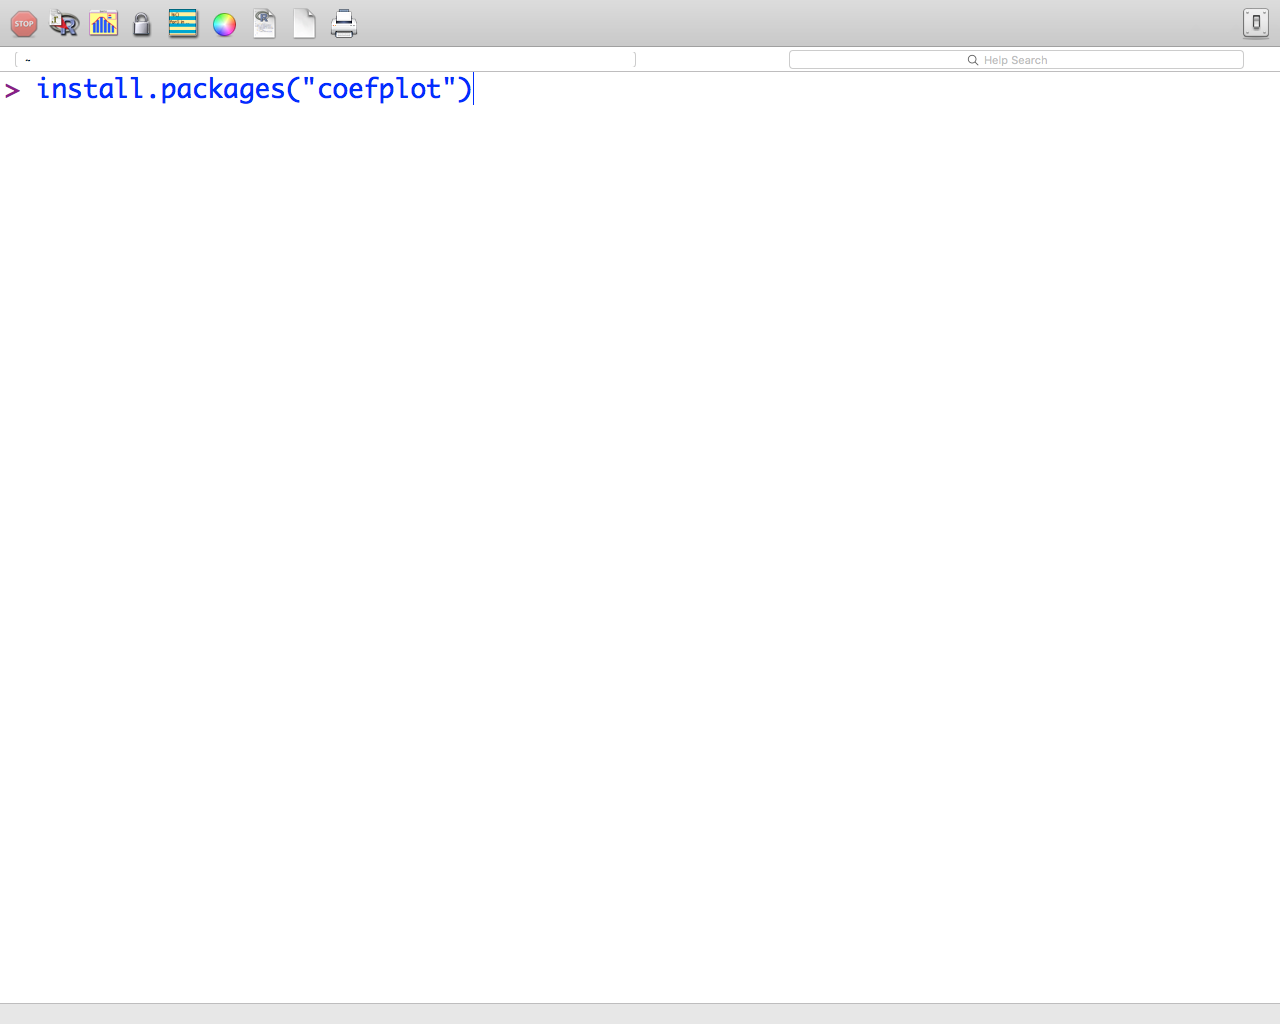
\includegraphics[width=\textwidth,height=0.75\textheight]{pic0014}\end{figure}
\end{frame}

\begin{frame}
\frametitle{Избор на сървър за изтегляне на пакета}
\begin{figure}[]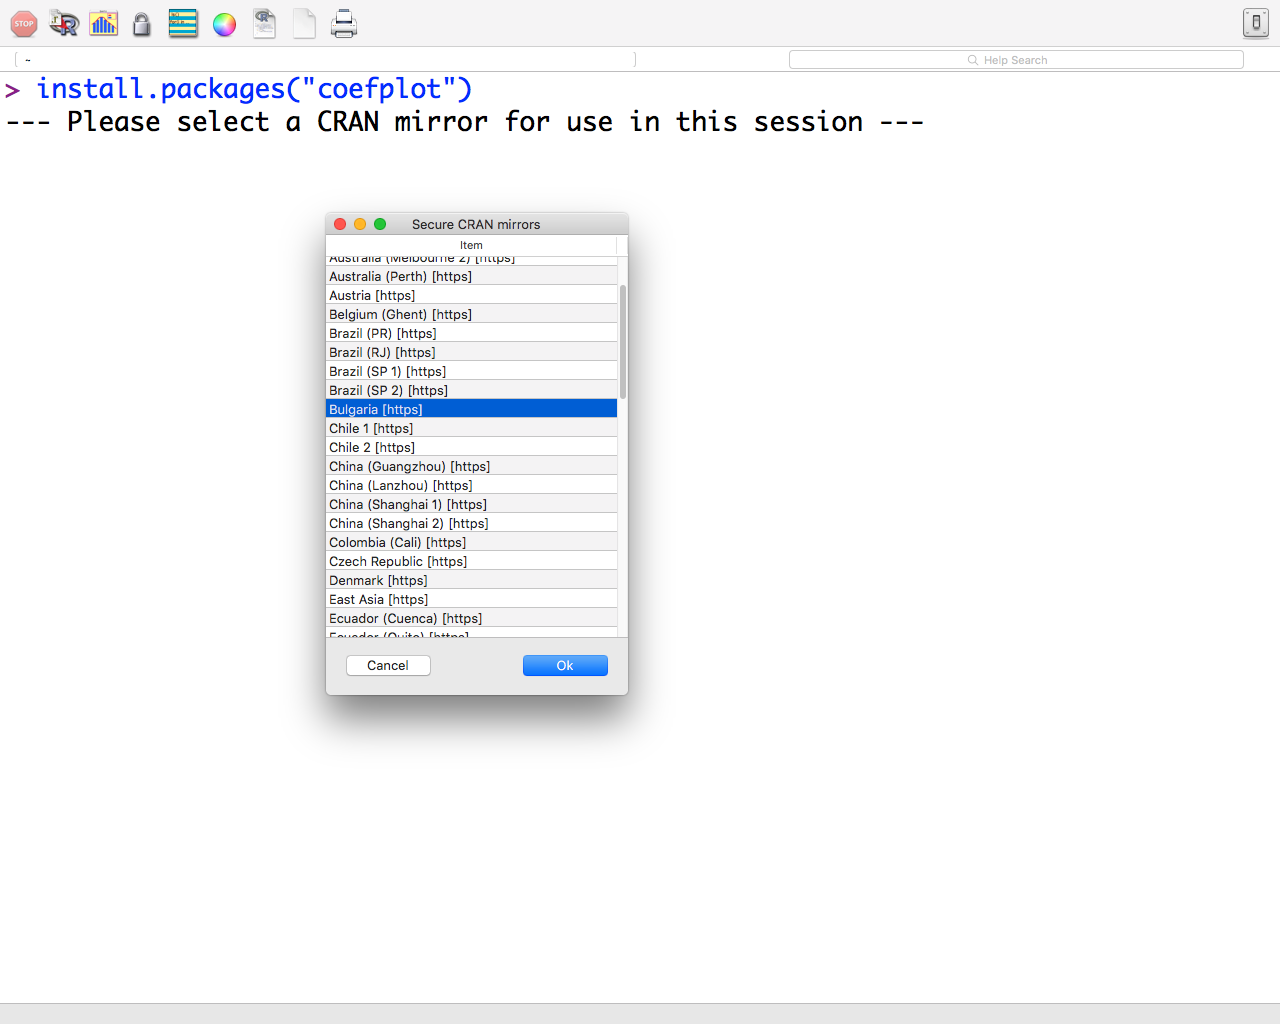
\includegraphics[width=\textwidth,height=0.75\textheight]{pic0015}\end{figure}
\end{frame}

\subsection{Връзки между пакетите}

\begin{frame}
\frametitle{Зависимости между пакетите}
\begin{figure}[]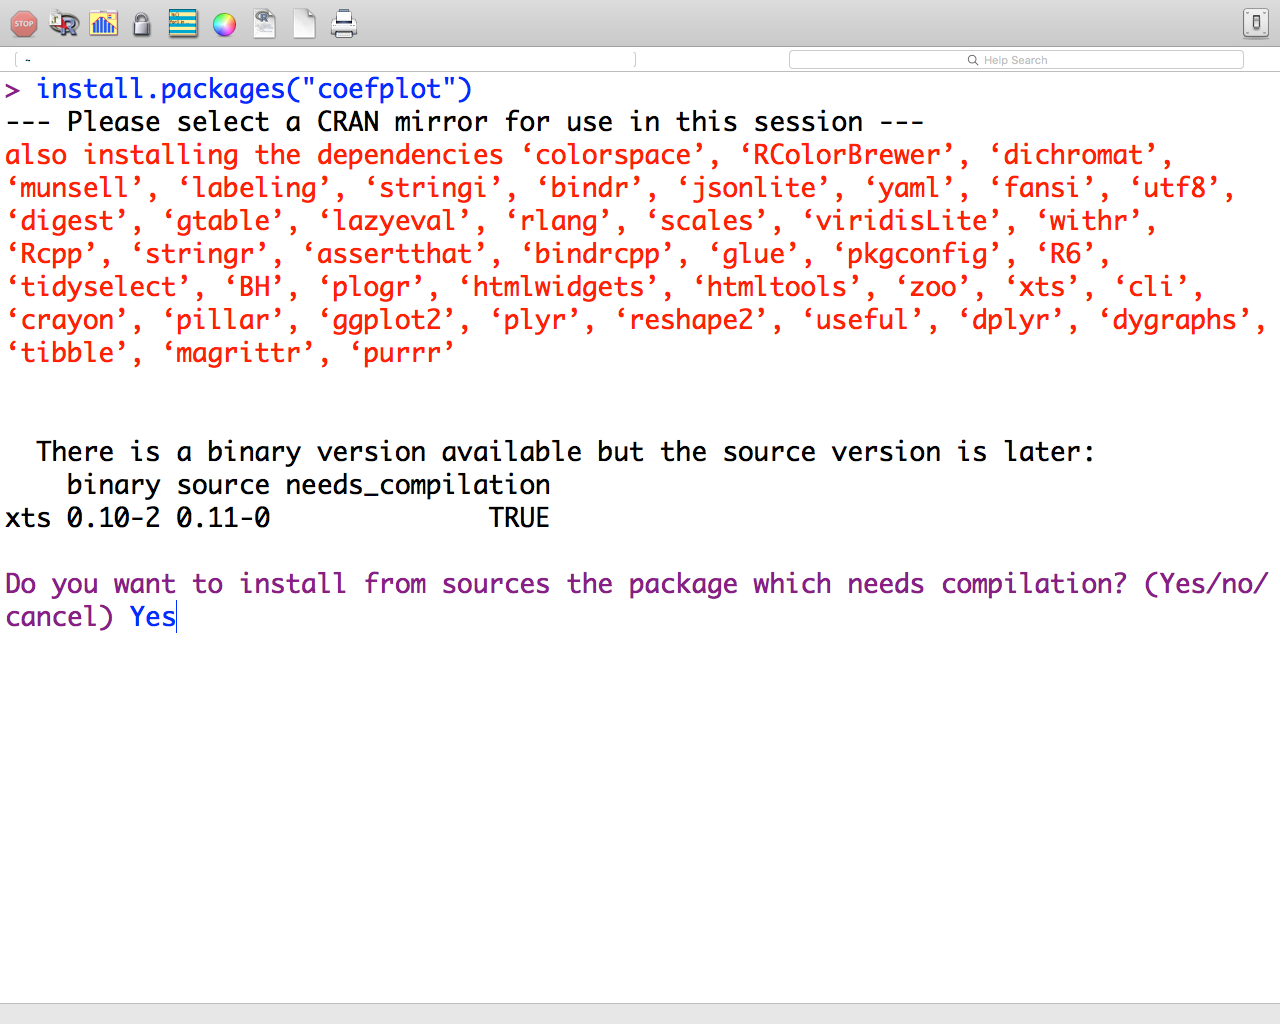
\includegraphics[width=\textwidth,height=0.75\textheight]{pic0016}\end{figure}
\end{frame}

\begin{frame}
\frametitle{Резултат от инсталацията на пакета}
\begin{figure}[]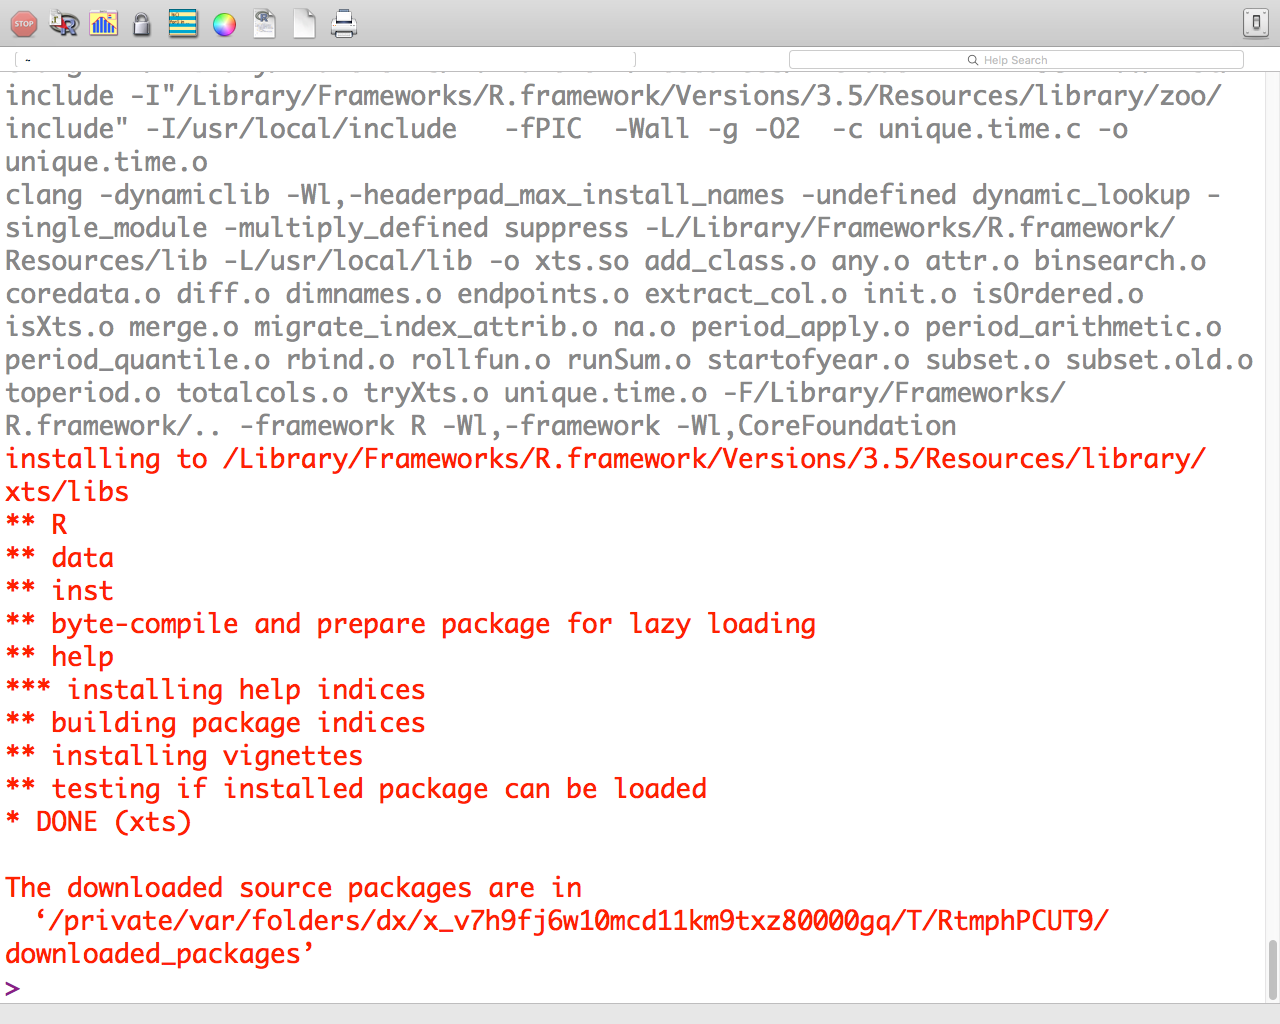
\includegraphics[width=\textwidth,height=0.75\textheight]{pic0017}\end{figure}
\end{frame}

\subsection{Зареждане и премахване на пакети}

\begin{frame}
\frametitle{Зареждане на пакета coefplot}
\begin{figure}[]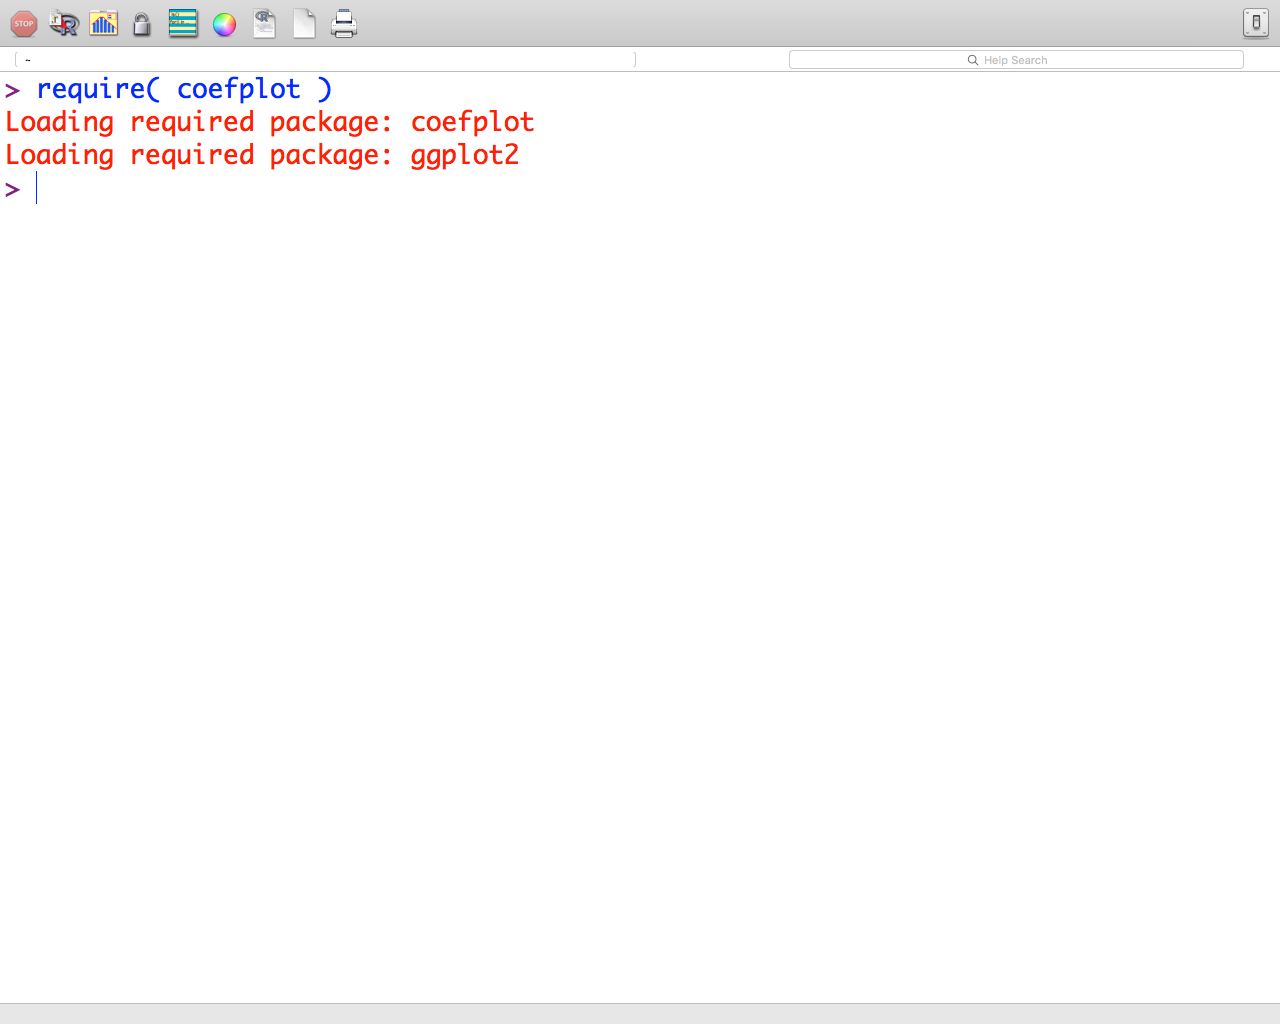
\includegraphics[width=\textwidth,height=0.75\textheight]{pic0018}\end{figure}
\end{frame}

\begin{frame}
\frametitle{Премахване на пакета coefplot от общата памет}
\begin{figure}[]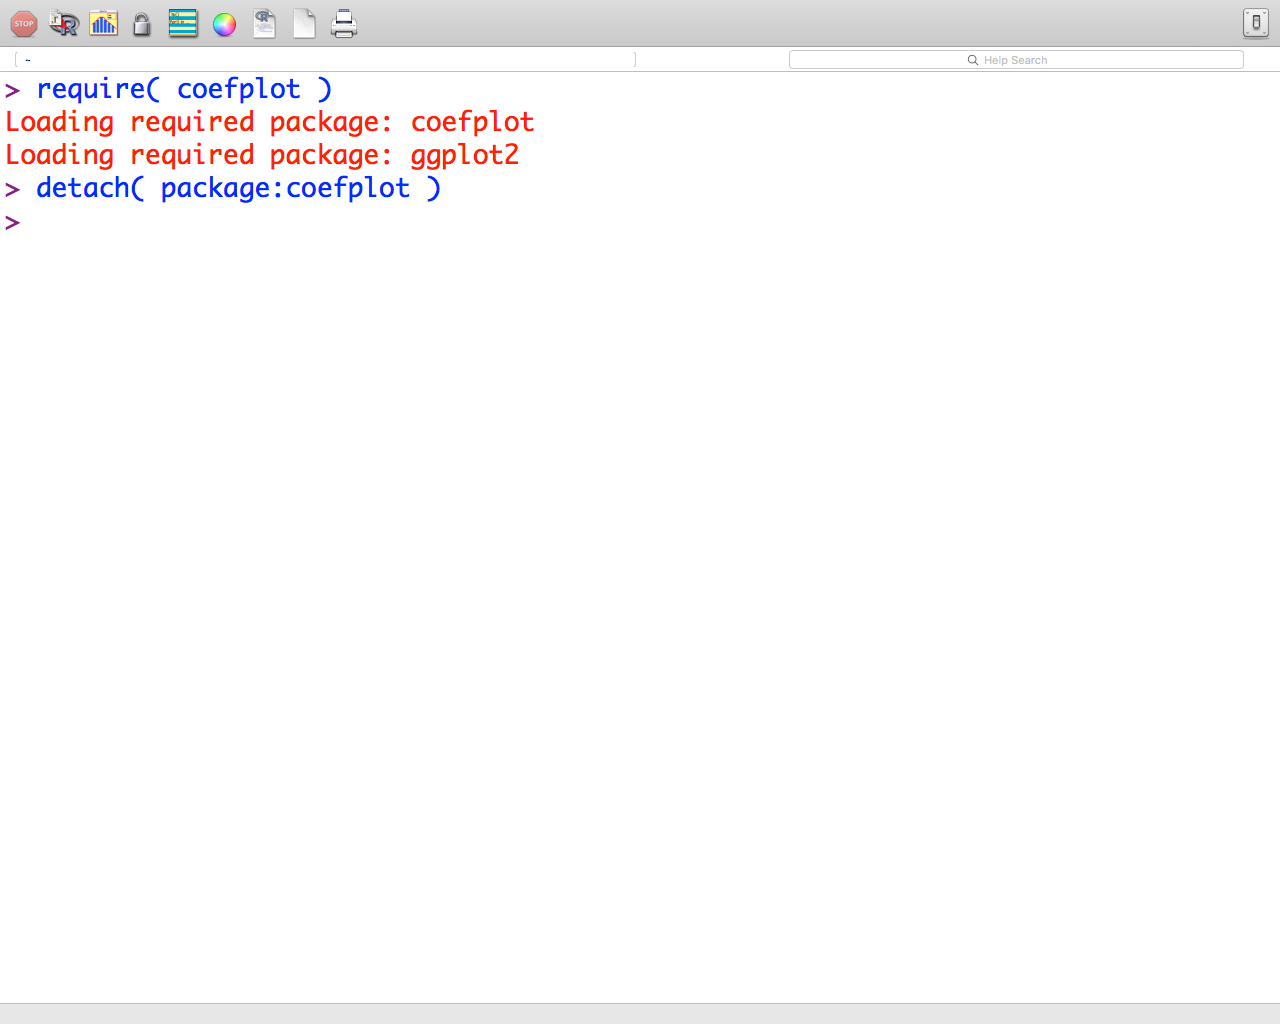
\includegraphics[width=\textwidth,height=0.75\textheight]{pic0019}\end{figure}
\end{frame}

\section{Основни математически операции}

\begin{frame}
\center \huge{Основни математически операции}
\end{frame}

\subsection{Изпълнение на команди с операции за пресмятане}

\begin{frame}
\frametitle{Примерни аритметични операции}
\begin{figure}[]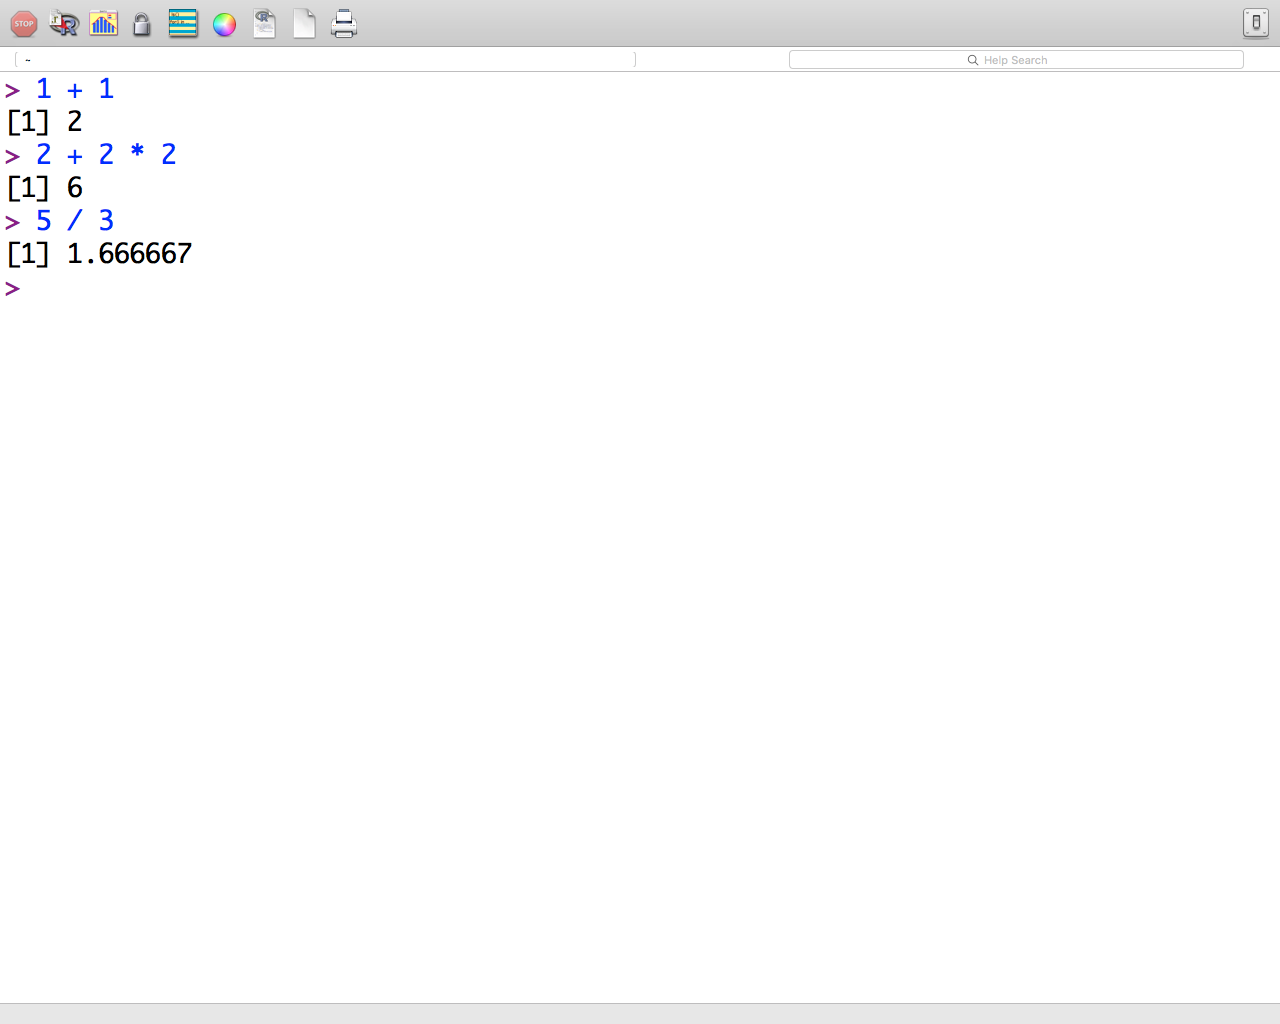
\includegraphics[width=\textwidth,height=0.75\textheight]{pic0020}\end{figure}
\end{frame}

\subsection{Свойства на операциите}

\begin{frame}
\frametitle{Кардиналност и асоциативност}
\begin{block}{Събиране - бинарна операция}
1 + 1
\end{block}
\begin{block}{Минус - унарна операция}
-5
\end{block}
\begin{block}{Лява асоциативност}
2 + 2 + 2
\end{block}
\begin{block}{Дясна асоциативност}
a = b = 2
\end{block}
\end{frame}

\begin{frame}
\frametitle{Контекстна зависимост на операциите}
\begin{block}{Контекстна зависимост при събиране}
"abc" + "def"

2 + 2
\end{block}
\begin{block}{Контекстна зависимост при делене}
5 / 3

5.0 / 3.0
\end{block}
\end{frame}

\begin{frame}
\frametitle{Приоритет на операциите}
\begin{block}{Аритметични операции}
2 + 2 * 2
\end{block}
\begin{block}{Смяна на приоритета}
(2 + 2) * 2
\end{block}
\end{frame}

\section{Типове и променливи}

\begin{frame}
\center \huge{Типове и променливи}
\end{frame}

\subsection{Създаване на променливи}

\begin{frame}
\frametitle{Операции за присвояване}
\begin{block}{Задаване на стойност}
a = 1

b <- 2

c = d = 3

e <- f <- 4

assign($"$g$"$, 5)

a += 6

b -= 7
\end{block}
\end{frame}

\begin{frame}
\frametitle{Алтернативи за присвояване}
\begin{block}{Два различни записа}
median(x = 1:10)

median(x <- 1:10)
\end{block}

В първия случай променливата x не остава в глобалната памет, а изчезва, докато при втория случай променливата x остава в глобалната памет след извикването.
\end{frame}

\subsection{Премахване на променливи}

\begin{frame}
\frametitle{Почистване на глобалната памет}
\begin{block}{Конкретна промелива или цялата памет}
rm( a )

rm( list=ls() )
\end{block}
\end{frame}

\section{Представяне на информацията}

\begin{frame}
\center \huge{Представяне на информацията}
\end{frame}

\subsection{Числени стойности}

\begin{frame}
\frametitle{Проверка за типа на променливата}
\begin{block}{Функция class}
a = 5

class( a )

[1] "numeric"
\end{block}

\begin{block}{Функция is.numeric}
is.numeric( a )

[1] TRUE
\end{block}
\end{frame}

\begin{frame}
\frametitle{Използване на целочислен тип}
\begin{block}{Типовете numeric и integer са различни}
b <- 6L

class( b )

[1] "integer"

is.numeric( b )

[1] TRUE

is.integer( b )

[1] TRUE

is.integer( a )

[1] FALSE
\end{block}
\end{frame}

\subsection{Символни низове}

\begin{frame}
\frametitle{Представяне на текст}
\begin{block}{Символни низове в R}
s1 <- "Simple text."

[1] "Simple text."

class( s1 )

[1] "character"

s2 <- factor( "Another simple text." )

[1] Another simple text.

Levels: Another simple text.

class( s2 )

[1] "factor"
\end{block}
\end{frame}

\begin{frame}
\frametitle{Дължина на данните}
\begin{block}{Символни низове и числа}
nchar( s1 )

[1] 12

nchar( s2 )

Error in nchar(s2) : 'nchar()' requires a character vector

nchar( a )

[1] 1
\end{block}
\end{frame}

\subsection{Астрономическо време}

\begin{frame}
\frametitle{Представяне на дати в паметта}
\begin{block}{Тип Date}
d1 <- as.Date("1979-04-21")

[1] "1979-04-21"

class( d1 )

[1] "Date"

as.numeric( d1 )

[1] 3397
\end{block}
\end{frame}

\begin{frame}
\frametitle{Представяне дати и часове в паметта}
\begin{block}{Тип POSIXct}
d2 <- as.POSIXct("1980-02-12 05:25")

[1] "1980-02-12 05:25:00 EET"

class( d2 )

[1] "POSIXct" "POSIXt" 

as.numeric( d2 )

[1] 319173900
\end{block}
\end{frame}

\subsection{Логически стойности}

\begin{frame}
\frametitle{Булеви стойности}
\begin{block}{Логически тип данни}
x1 <- TRUE

[1] TRUE

class( x1 )

[1] "logical"

is.logical( x1 )

[1] TRUE

as.numeric( x1 )

[1] 1
\end{block}
\end{frame}

\begin{frame}
\frametitle{Алтернативни константи}
\begin{block}{По-добре е да се ползва пълният запис}
x2 <- F

[1] FALSE

class( x2 )

[1] "logical"

is.logical( x2 )

[1] TRUE

as.numeric( x2 )

[1] 0
\end{block}
\end{frame}

\begin{frame}
\frametitle{Резултат от логически ирази}
\begin{block}{Операции за сравнение}
2 == 3

[1] FALSE

5 != 6

[1] TRUE

$"$Peter$"$ == $"$Ivan$"$

[1] FALSE
\end{block}
\end{frame}

\section{Заключение}

\begin{frame}
\center \huge{Заключение}
\end{frame}

\subsection{Дискусия}

\begin{frame}
\frametitle{Въпроси и отговори}
\center \huge{Благодаря за вниманието!}
\end{frame}

\end{document}
